\documentclass{article}
% translate with >> pdflatex -shell-escape <file>

% This file is used as unit test for pgfplots, copyright by Christian Feuersaenger.
% 
% See
%   http://pgfplots.sourceforge.net/pgfplots.pdf
% for pgfplots.
%
% Any required input files (for <plot table> or <plot file> or the table package) can be downloaded
% at
% http://www.ctan.org/tex-archive/graphics/pgf/contrib/pgfplots/doc/latex/
% and
% http://www.ctan.org/tex-archive/graphics/pgf/contrib/pgfplots/doc/latex/plotdata/

\usepackage{pgfplotstable}
\usepackage{longtable}
\pgfplotsset{compat=newest}

\pagestyle{empty}


\begin{document}

{
	\def\testit#1#2{%
		\begingroup
		\pgfplotsutilstrcmp{#1}{#2}%
		\ttfamily #1 \ifcase\pgfplotsretval =\or<\or>\fi\space #2 
		\endgroup
		\par
	}%

	\testit{z}{aaa}
	\testit{A longer Test}{A longer verification}
	\testit{a}{a}
	\testit{a}{b}
	\testit{b}{a}
	\testit{aa}{ab}
	\testit{aba}{abb}
	\testit{eins}{zwei}
	\testit{vier}{fuenf}

	\pgfplotstableread{
		The
		values
		of
		these
		keys
		contain
		the
		size
		of
		the
		parent
		axis.
		They
		can
		be
		used
		as
		|width|
		and/or
		|height|
		arguments
		for
		|every
		colorbar|
		with
		|\pgfkeysvalueof{/pgfplots/parent
		axis
		width}|.
		These
		values
		are
		only
		valid
		inside
		of
		color
		bars.
		\end{pgfplotskeylist}
		Besides
		these
		values,
		each
		color
		bar
		inherits
		a
		list
		of
		styles
		of
		its
		parent
		axis,
		namely
		\begin{itemize}
		\item
		|every
		tick|,
		\item
		|every
		minor
		tick|,
		\item
		|every
		major
		tick|,
		\item
		|every
		axis
		grid|,
		\item
		|every
		minor
		grid|,
		\item
		|every
		major
		grid|,
		\item
		|every
		tick
		label|.
		\end{itemize}
		This
		can
		be
		used
		to
		inherit
		line
		width
		and/or
		fonts.
		\begin{codeexample}[]
		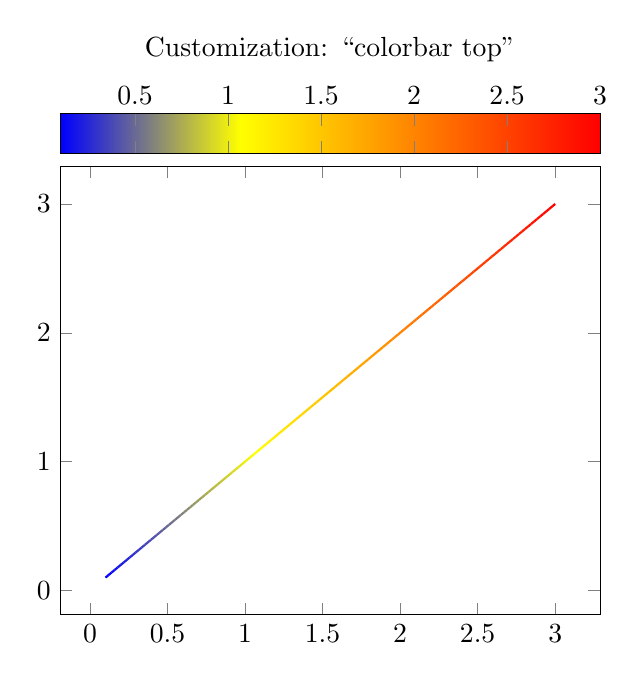
\begin{tikzpicture}
		\begin{axis}[
		colorbar
		horizontal,
		colorbar
		style={
		at={(0.5,1.03)},anchor=south,
		xticklabel
		pos=upper
		},
		title
		style={yshift=1cm},
		title=Customization:
		``colorbar
		top'']
		\addplot[mesh,thick,samples=150,domain=0.1:3]
		{x};
		\end{axis}
		\end{tikzpicture}
		\end{codeexample}
		\begin{codeexample}[]
		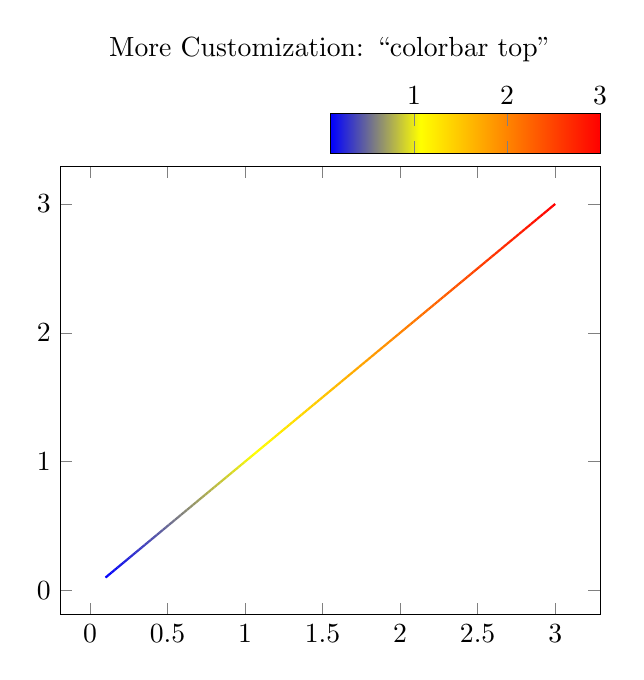
\begin{tikzpicture}
		\begin{axis}[
		colorbar
		horizontal,
		colorbar
		style={
		at={(1,1.03)},anchor=south
		east,
		width=0.5*
		\pgfkeysvalueof{/pgfplots/parent
		axis
		width},
		xticklabel
		pos=upper,
		},
		title
		style={yshift=1cm},
		title=More
		Customization:
		``colorbar
		top'']
		\addplot[mesh,thick,samples=150,domain=0.1:3]
		{x};
		\end{axis}
		\end{tikzpicture}
		\end{codeexample}
		Please
		take
		a
		look
		at
		the
		predefined
		styles
		|colorbar
		right|,
		|colorbar
		left|
		and
		|colorbar
		horizontal|
		for
		more
		details
		about
		configuration
		possibilities
		for
		|every
		colorbar|.
		\paragraph{Remark:}
		A
		color
		bar
		is
		just
		a
		normal
		axis.
		That
		means
		|every
		colorbar|
		can
		contain
		specifications
		where
		to
		place
		tick
		labels,
		extra
		ticks,
		scalings
		and
		most
		other
		features
		of
		a
		normal
		axis
		as
		well
		(except
		nested
		color
		bars).
	}\loadedtable

	\ttfamily
	\pgfplotstablesort[sort cmp={string <}]\loadedtable\loadedtable
	
	%\tracingmacros=2 \tracingcommands=2

	\onecolumn

	\subsection{A sorted crap table}

	\pgfplotstabletypeset[column type=l,begin table=\begin{longtable},end table=\end{longtable},verb string type]\loadedtable

	\twocolumn
}
\end{document}

